% 2001 年全国新课程卷理科第 21 题：冷却塔双曲线截面
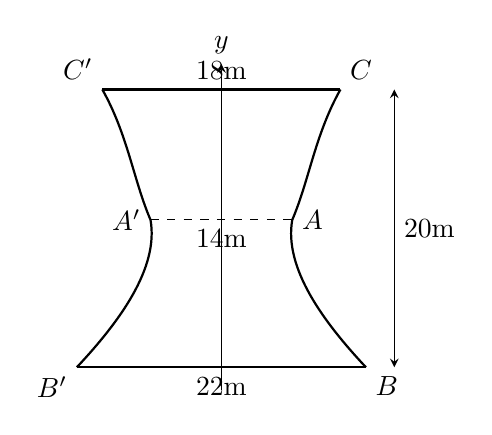
\begin{tikzpicture}[>=stealth, scale=0.72]
  \coordinate (TL) at (-2.1,2.45);
  \coordinate (TR) at (2.1,2.45);
  \coordinate (ML) at (-1.25,0.15);
  \coordinate (MR) at (1.25,0.15);
  \coordinate (BL) at (-2.55,-2.45);
  \coordinate (BR) at (2.55,-2.45);

  \draw[thick] (TL) .. controls (-1.65,1.65) and (-1.55,0.85) .. (ML)
    .. controls (-1.1,-0.7) and (-1.8,-1.65) .. (BL);
  \draw[thick] (TR) .. controls (1.65,1.65) and (1.55,0.85) .. (MR)
    .. controls (1.1,-0.7) and (1.8,-1.65) .. (BR);
  \draw[thick] (TL)--(TR) node[midway, above] {$18\mathrm{m}$};
  \draw[thick] (BL)--(BR) node[midway, below] {$22\mathrm{m}$};
  \draw[dashed] (ML)--(MR) node[midway, below] {$14\mathrm{m}$};
  \draw[<->] (3.05,-2.45)--(3.05,2.45) node[midway, right] {$20\mathrm{m}$};
  \draw[->] (0,-2.85)--(0,2.9) node[above] {$y$};
  \node[above left] at (TL) {$C'$};
  \node[above right] at (TR) {$C$};
  \node[left] at (ML) {$A'$};
  \node[right] at (MR) {$A$};
  \node[below left] at (BL) {$B'$};
  \node[below right] at (BR) {$B$};
\end{tikzpicture}
